\documentclass[aspectratio=169]{beamer}

% Theme Selection
\usetheme{Madrid}
\usecolortheme{default}
\usefonttheme{structurebold}

% Packages
\usepackage{amsmath}
\usepackage{amssymb}
\usepackage{graphicx}
\usepackage{booktabs}
\usepackage{tikz}
\usepackage{caption}

% Title Information
\title[Neural Metropolis-Hastings]{Neural Metropolis-Hastings: \\ MCMC Sampling with Learned Proposals}
\subtitle{Numerical Methods Project}
\author{Hao Luo}
\date{\today}

% Begin Document
\begin{document}

% Title Slide
\begin{frame}
    \titlepage
\end{frame}

% Outline
% \begin{frame}{Outline}
%     \tableofcontents
% \end{frame}

\AtBeginSection[]{
  \begin{frame}
    \frametitle{Outline}
    \tableofcontents[currentsection]
  \end{frame}
}

% ---------------------------------------------------------
% SECTION 1: Introduction
% ---------------------------------------------------------
\section{Introduction to MCMC}

\begin{frame}{The Sampling Problem}
    \begin{block}{Goal}
        Generate independent samples $\{x_i\}_{i=1}^R$ from a target distribution $P(x)$.
    \end{block}
    
    \vspace{0.5cm}
    
    \begin{itemize}
        \item Target distribution is often known only up to a constant:
        $$ P(x) = \frac{\tilde{P}(x)}{Z}, \quad Z = \int \tilde{P}(x) dx $$
        \item \textbf{Challenge:} The "Curse of Dimensionality."
        \item In high dimensions, finding modes and exploring the space becomes exponentially difficult.
        \item Standard methods often get stuck in local modes.
    \end{itemize}
\end{frame}

\begin{frame}{Metropolis-Hastings (MH) Algorithm}
    \begin{itemize}
        \item A Markov Chain Monte Carlo (MCMC) method.
        \item Constructs a chain with equilibrium distribution $P(x)$.
        \item \textbf{Two Steps per Iteration:}
        \begin{enumerate}
            \item \textbf{Proposal:} Sample candidate $x'$ from $Q(x'|x^{(t)})$.
            \item \textbf{Acceptance:} Accept $x'$ with probability $\alpha$:
        \end{enumerate}
    \end{itemize}
    
    \begin{equation*}
        \alpha = \min\left(1, \frac{P(x') Q(x^{(t)}|x')}{P(x^{(t)}) Q(x'|x^{(t)})}\right)
    \end{equation*}
    
    \vspace{0.2cm}
    \footnotesize{Ensures \textbf{Detailed Balance}: $\pi(x)T(x \to y) = \pi(y)T(y \to x)$}
\end{frame}

\begin{frame}{Challenges of Classical MH}
    Classical MH uses a \textbf{fixed-step} Gaussian proposal: $Q = \mathcal{N}(x_t, \sigma^2 I)$.
    
    \vspace{0.3cm}
    
    \begin{columns}
        \column{0.5\textwidth}
        \textbf{1. Slow Convergence}
        \begin{itemize}
            \item Random walk behavior.
            \item Steps $\epsilon$ require $O((L/\epsilon)^2)$ steps to explore region $L$.
        \end{itemize}
        
        \column{0.5\textwidth}
        \textbf{2. High Correlation}
        \begin{itemize}
            \item Poorly chosen $\sigma$ leads to highly correlated samples.
            \item Reduces Effective Sample Size (ESS).
        \end{itemize}
    \end{columns}
    
    \vspace{0.5cm}
    \begin{alertblock}{Insight}
        Instead of a blind random walk, we give the walker \textbf{"eyes"}: a Neural Network that learns the local geometry to take smarter steps.
    \end{alertblock}
\end{frame}

% ---------------------------------------------------------
% SECTION 2: Methodology
% ---------------------------------------------------------
\section{Neural Metropolis-Hastings}

\begin{frame}{Model Formulation}
    We parameterize the proposal covariance using a Neural Network (MLP).
    
    \begin{equation*}
        Q_\theta(x'|x^{(t)}) = \mathcal{N}\left(x'; x^{(t)}, \boldsymbol{\Sigma}_\theta(x^{(t)})\right)
    \end{equation*}
    
    \begin{itemize}
        \item $\boldsymbol{\Sigma}_\theta(x) = \text{diag}(\sigma_1^2(x), \dots, \sigma_d^2(x))$.
        \item Input: Current state $x^{(t)}$.
        \item Output: Log-variances for each dimension $\log \sigma_i^2(x)$.
        \item \textbf{Key Feature:} State-dependent step sizes.
    \end{itemize}
\end{frame}

\begin{frame}{Loss Function Design}
    Goal: Minimize KL-Divergence between Proposal $Q_\theta$ and Target $P$.
    
    $$
    \begin{aligned}
    \mathcal{L}(\theta) &= \text{KL}(Q_\theta( \cdot |x^{(t)}) || P(\cdot)) \\
    &= \int Q_\theta(x'|x^{(t)}) \log \frac{Q_\theta(x'|x^{(t)})}{P(x')} dx' \\
    &= -\int Q_\theta(x'|x^{(t)}) \log P(x') dx' + \int Q_\theta(x'|x^{(t)}) \log Q_\theta(x'|x^{(t)}) dx' \\
    \end{aligned}
    $$
    
    \vspace{0.3cm}
    \textbf{Monte Carlo Estimate for Batch $\{x'_i\}$:}
    $$ \mathcal{L}(\theta) \approx -\frac{1}{N} \sum_{i=1}^N \Big[\log \tilde{P}(x'_i) + H(Q_\theta(x^{(t)}_i))\Big] $$
    
    \begin{itemize}
        \item \textbf{Energy Term:} Pushes proposals toward high-probability regions.
        \item \textbf{Entropy Term:} Prevents variance collapse (encourages exploration).
        \item \textbf{Note:} The prior probability $P(x')$ is implicitly included by the sampling process.
    \end{itemize}
\end{frame}

\begin{frame}{Training Procedure}
    \begin{enumerate}
        \item \textbf{Warm-up Phase:}
        \begin{itemize}
            \item Run classical MH with fixed $\sigma$.
            \item Generates initial data to stabilize the network.
        \end{itemize}
        
        \vspace{0.2cm}
        
        \item \textbf{Online Training Phase:}
        \begin{itemize}
            \item Switch to Neural Proposal.
            \item Update network weights iteratively after each batch.
            \item Uses \textbf{Reparameterization Trick} for differentiable sampling.
        \end{itemize}
    \end{enumerate}
\end{frame}

% ---------------------------------------------------------
% SECTION 3: Experiments
% ---------------------------------------------------------
\section{Experiments and Results}

\begin{frame}{Experimental Setup}
    \textbf{Target Distribution:} Himmelblau's Function (Boltzmann Distribution)
    
    $$ f(x) = (x_1^2 + x_2 - 11)^2 + (x_1 + x_2^2 - 7)^2 $$
    $$ P(x) \propto \exp(-f(x) / T), \quad T=20 $$
    
    \begin{figure}
        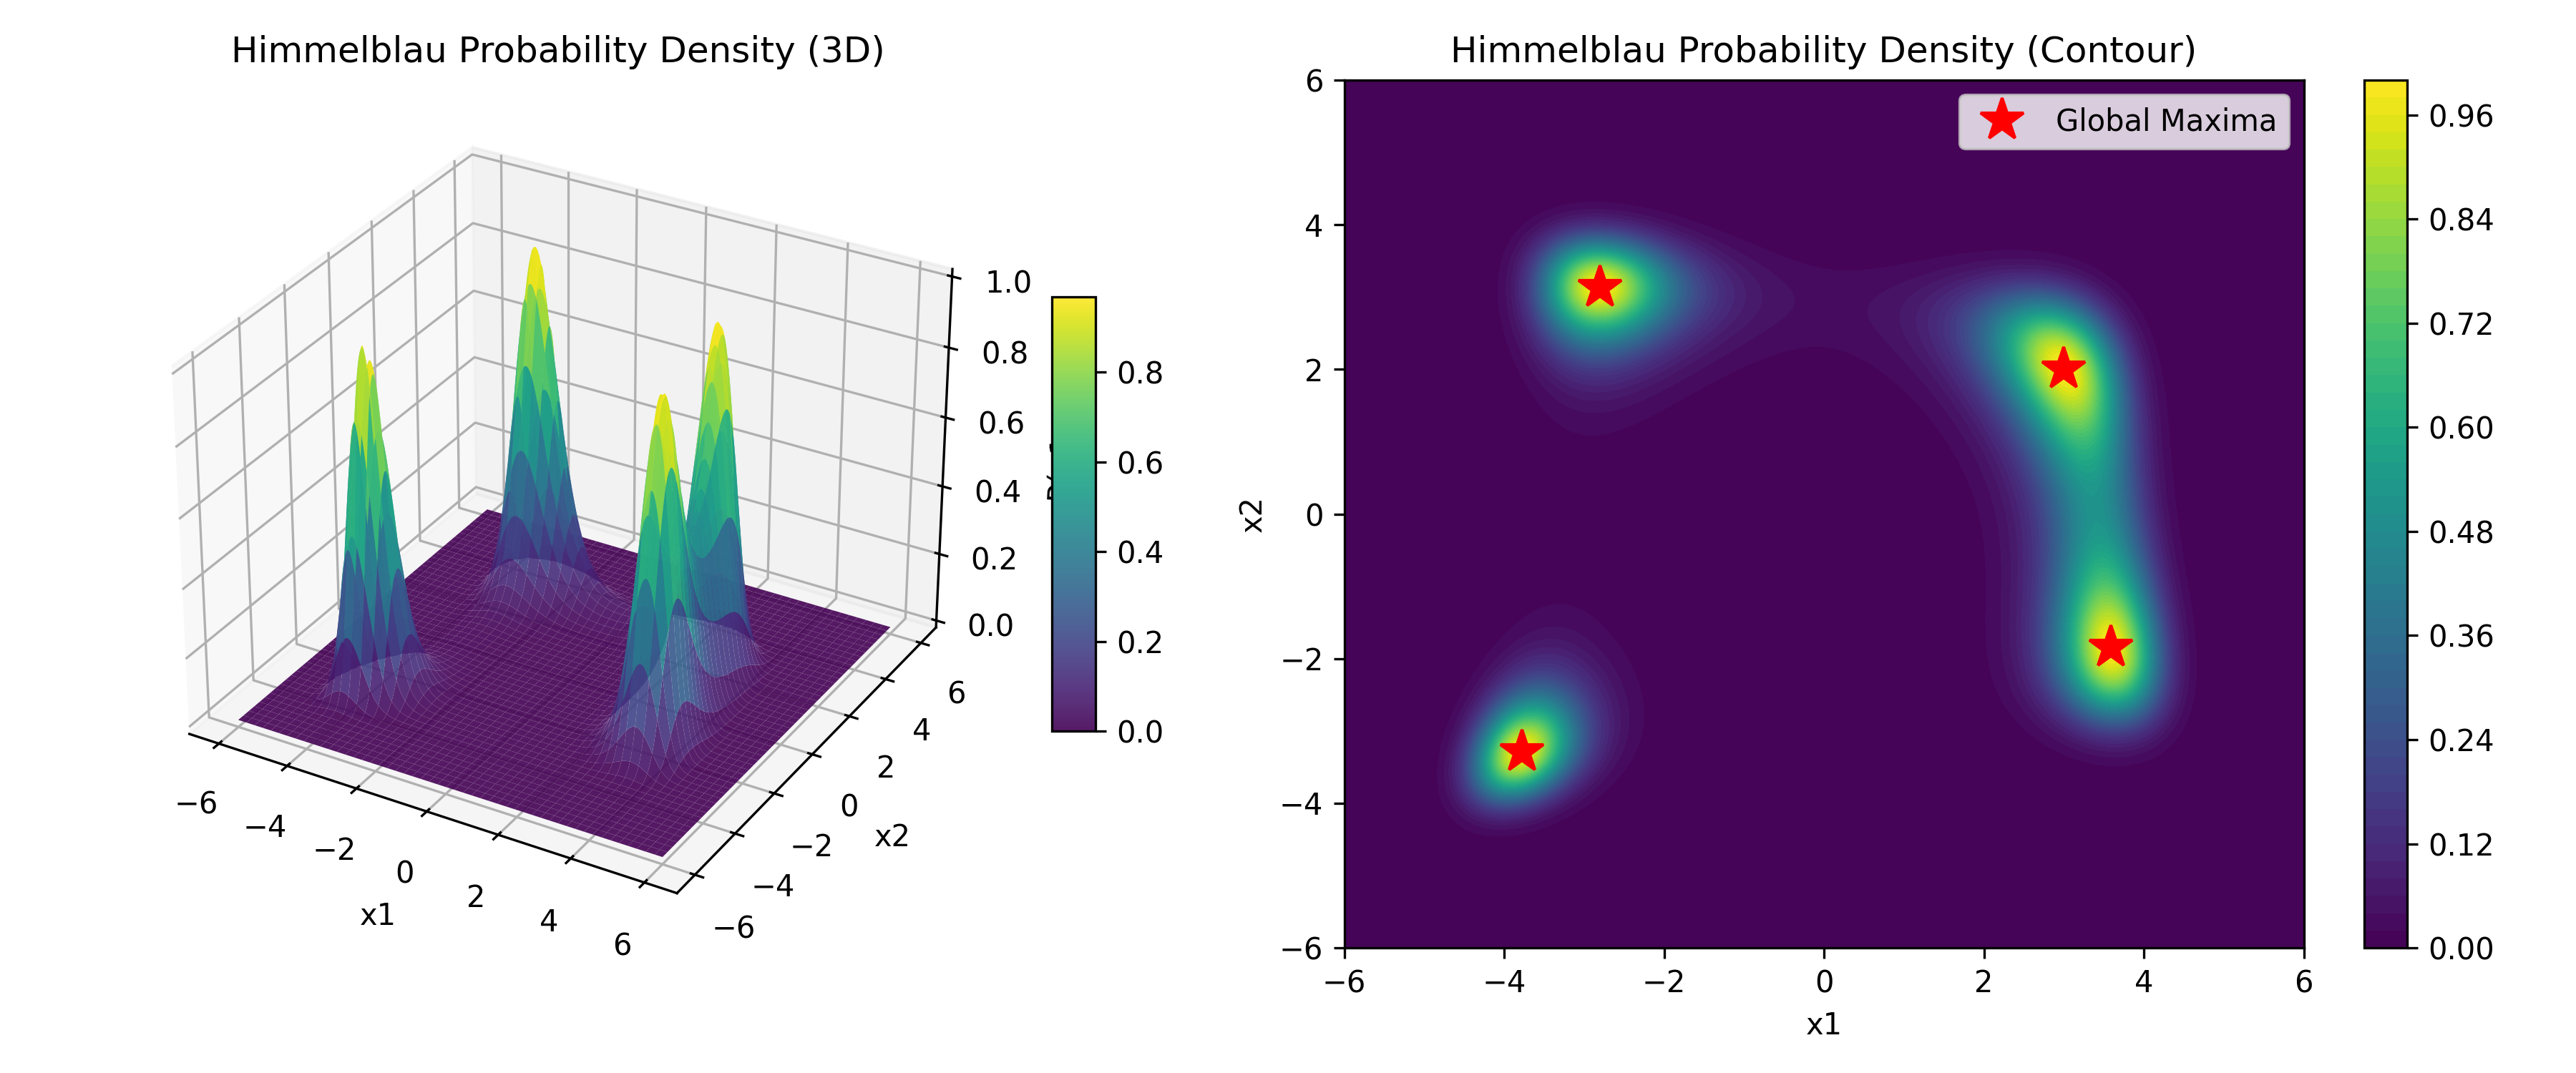
\includegraphics[width=0.7\textwidth]{../assets/himmelblau_density.png}
        \caption{Target Density}
    \end{figure}
\end{frame}

\begin{frame}{Classical MH Performance}
    \textbf{Settings:} Fixed $\sigma=1.0$, 10,000 iterations.
    
    \begin{columns}
        \column{0.4\textwidth}
        \begin{figure}
            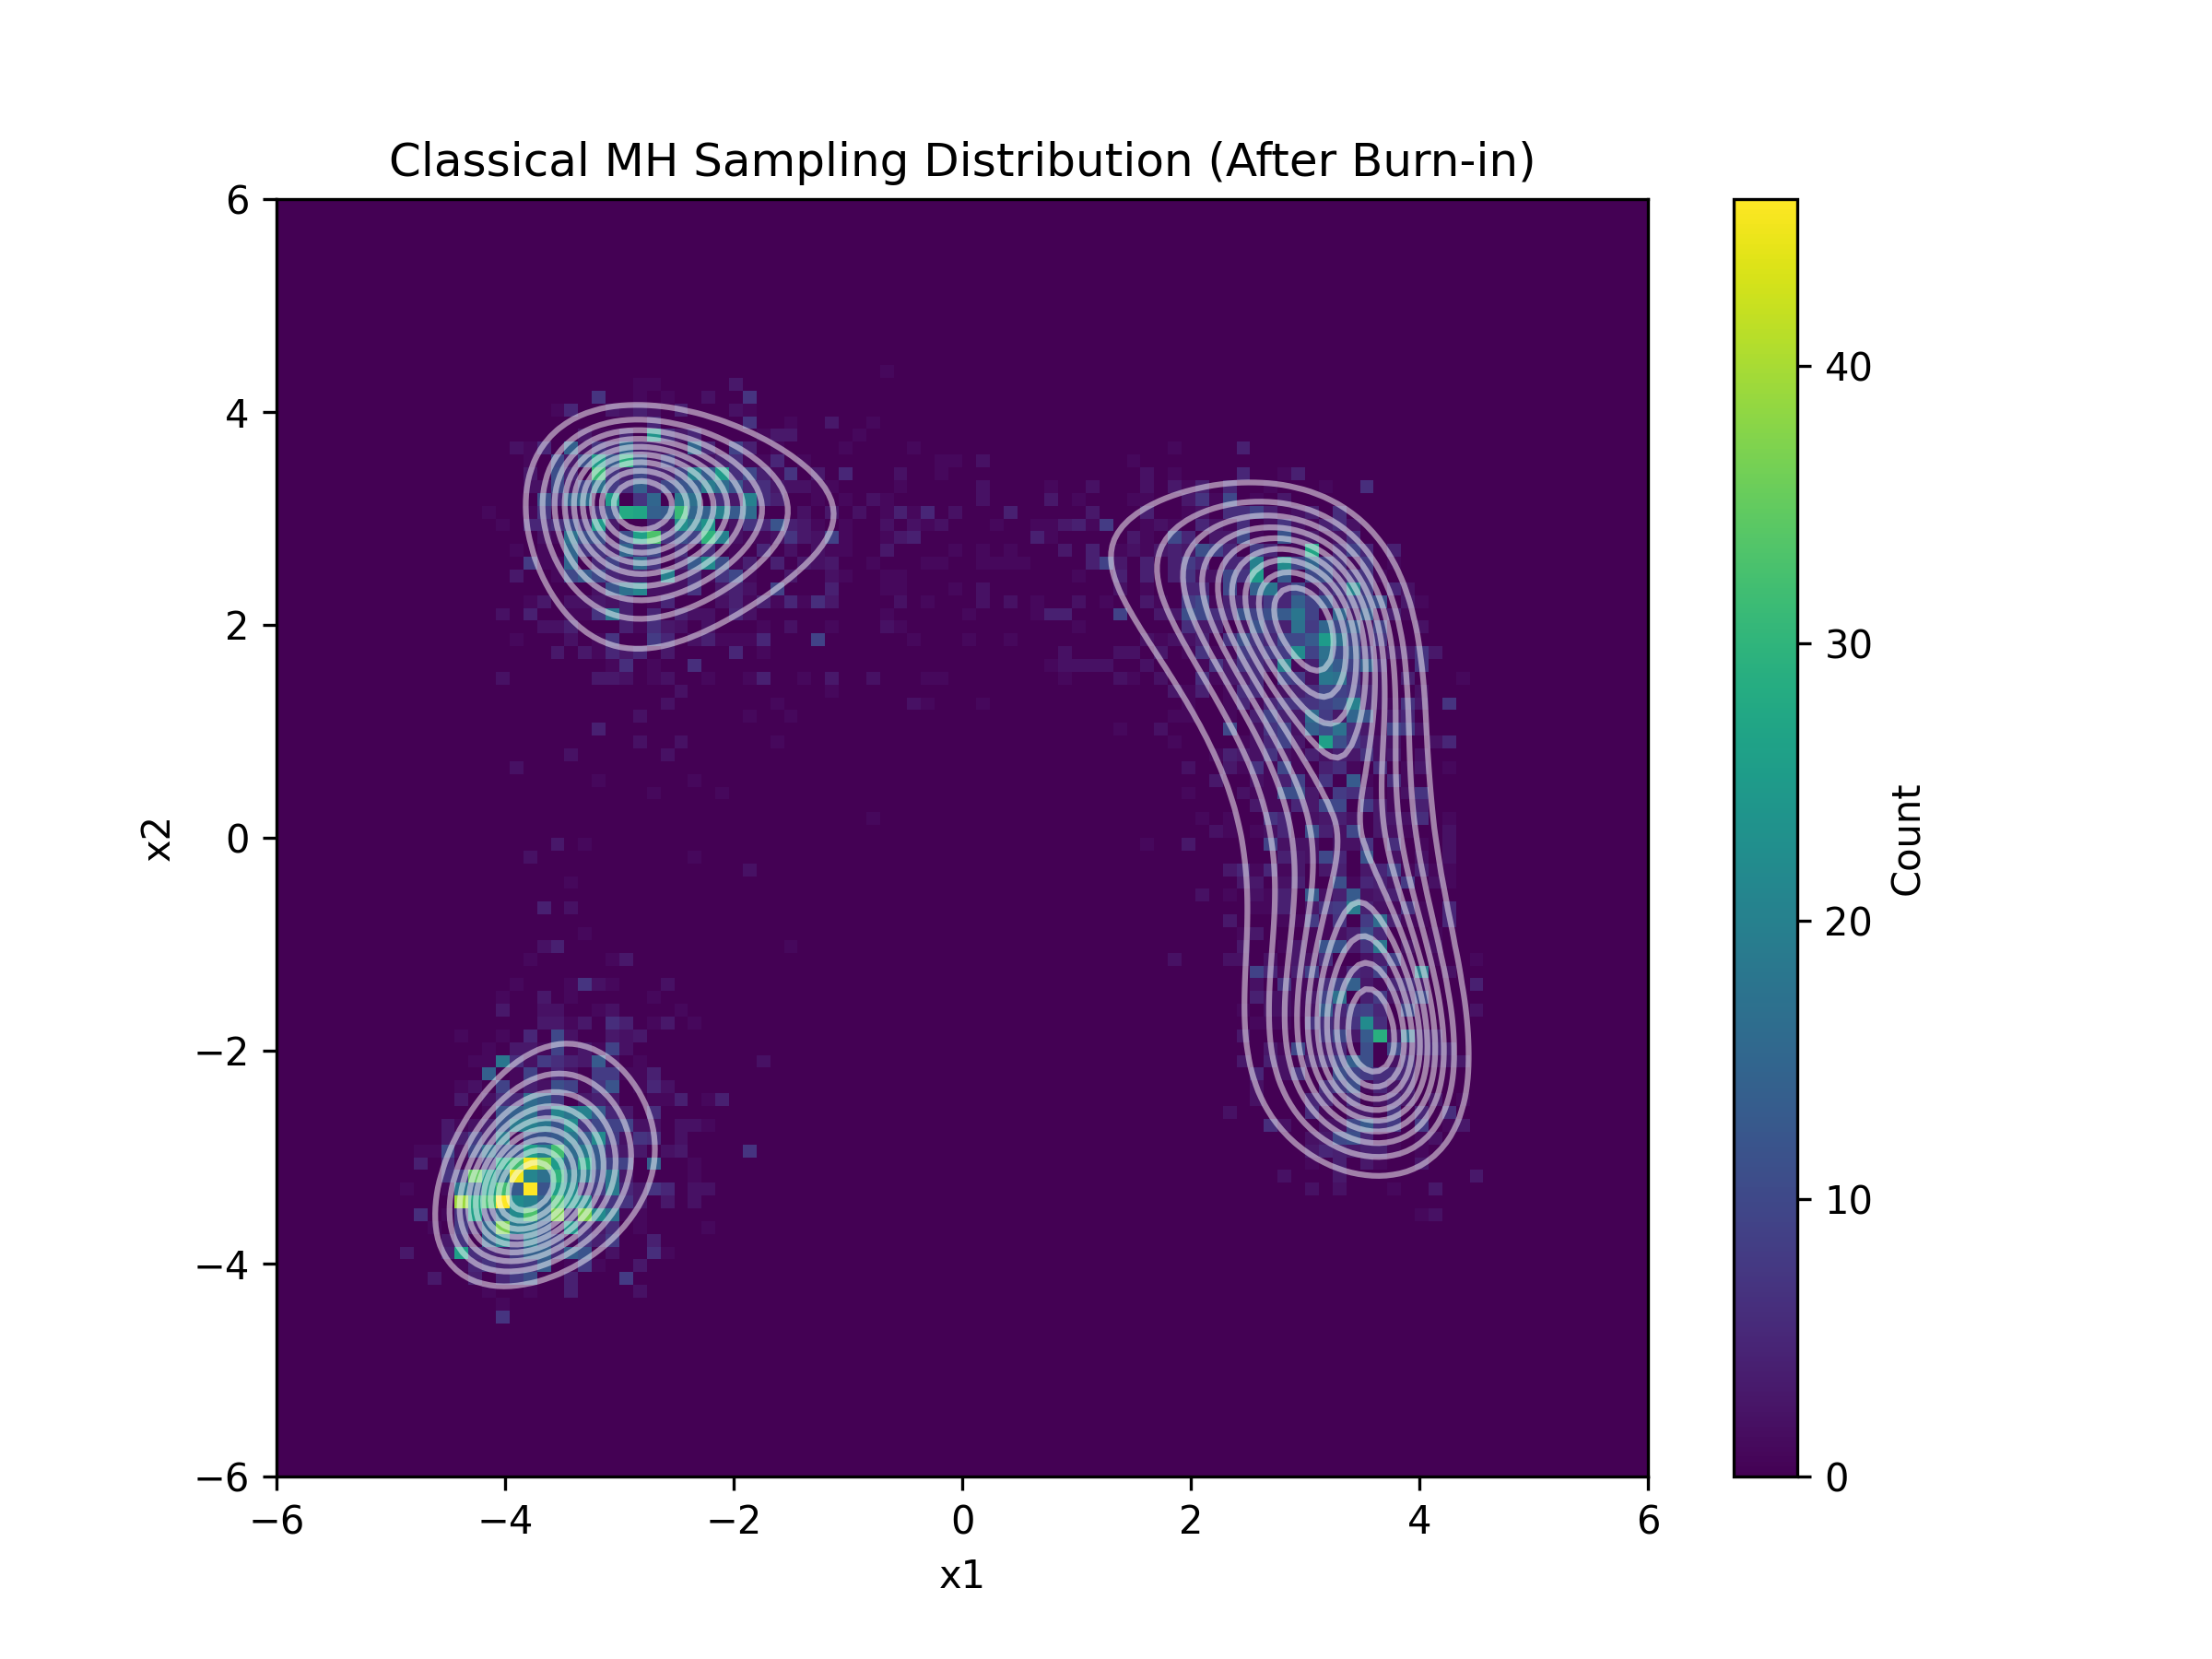
\includegraphics[width=\textwidth]{../assets/classical_hist2d.png}
            \caption{2D Histogram}
        \end{figure}
        
        \column{0.6\textwidth}
        \begin{figure}
            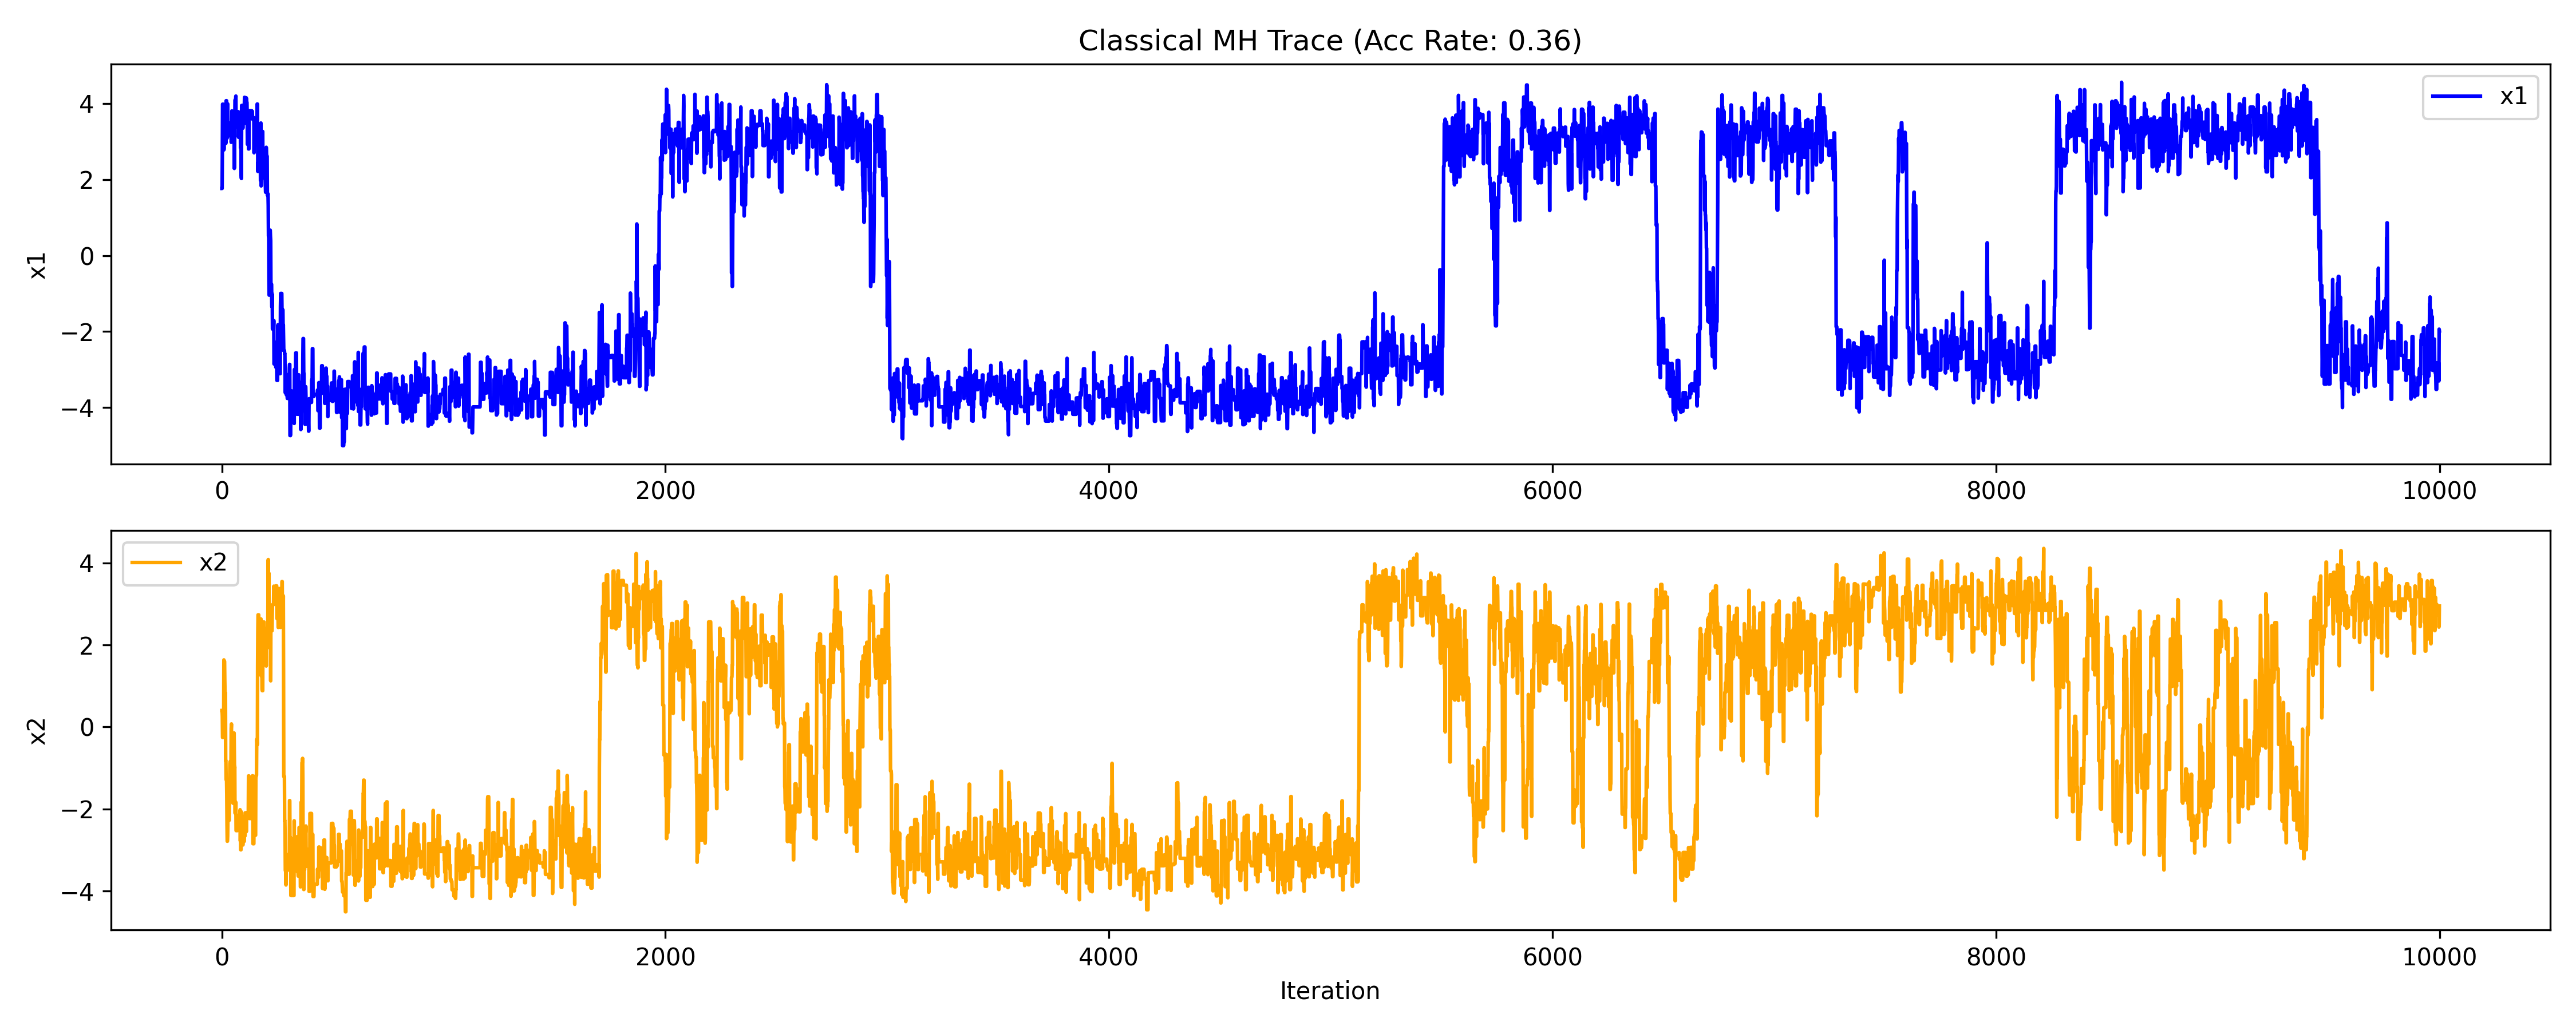
\includegraphics[width=\textwidth]{../assets/classical_trace.png}
            \caption{Trace Plot}
        \end{figure}
    \end{columns}
    
    \begin{itemize}
        \item Acceptance Rate: $\approx 0.4$.
        \item \textbf{Result:} Gets stuck in the left-bottom mode.
        \item Fails to explore all 4 modes evenly within 10k steps.
    \end{itemize}
\end{frame}

\begin{frame}{Neural MH: Training Dynamics}
    \textbf{Settings:} 20k iterations (2k warm-up), $\beta=1.0$.
    
    \begin{figure}
        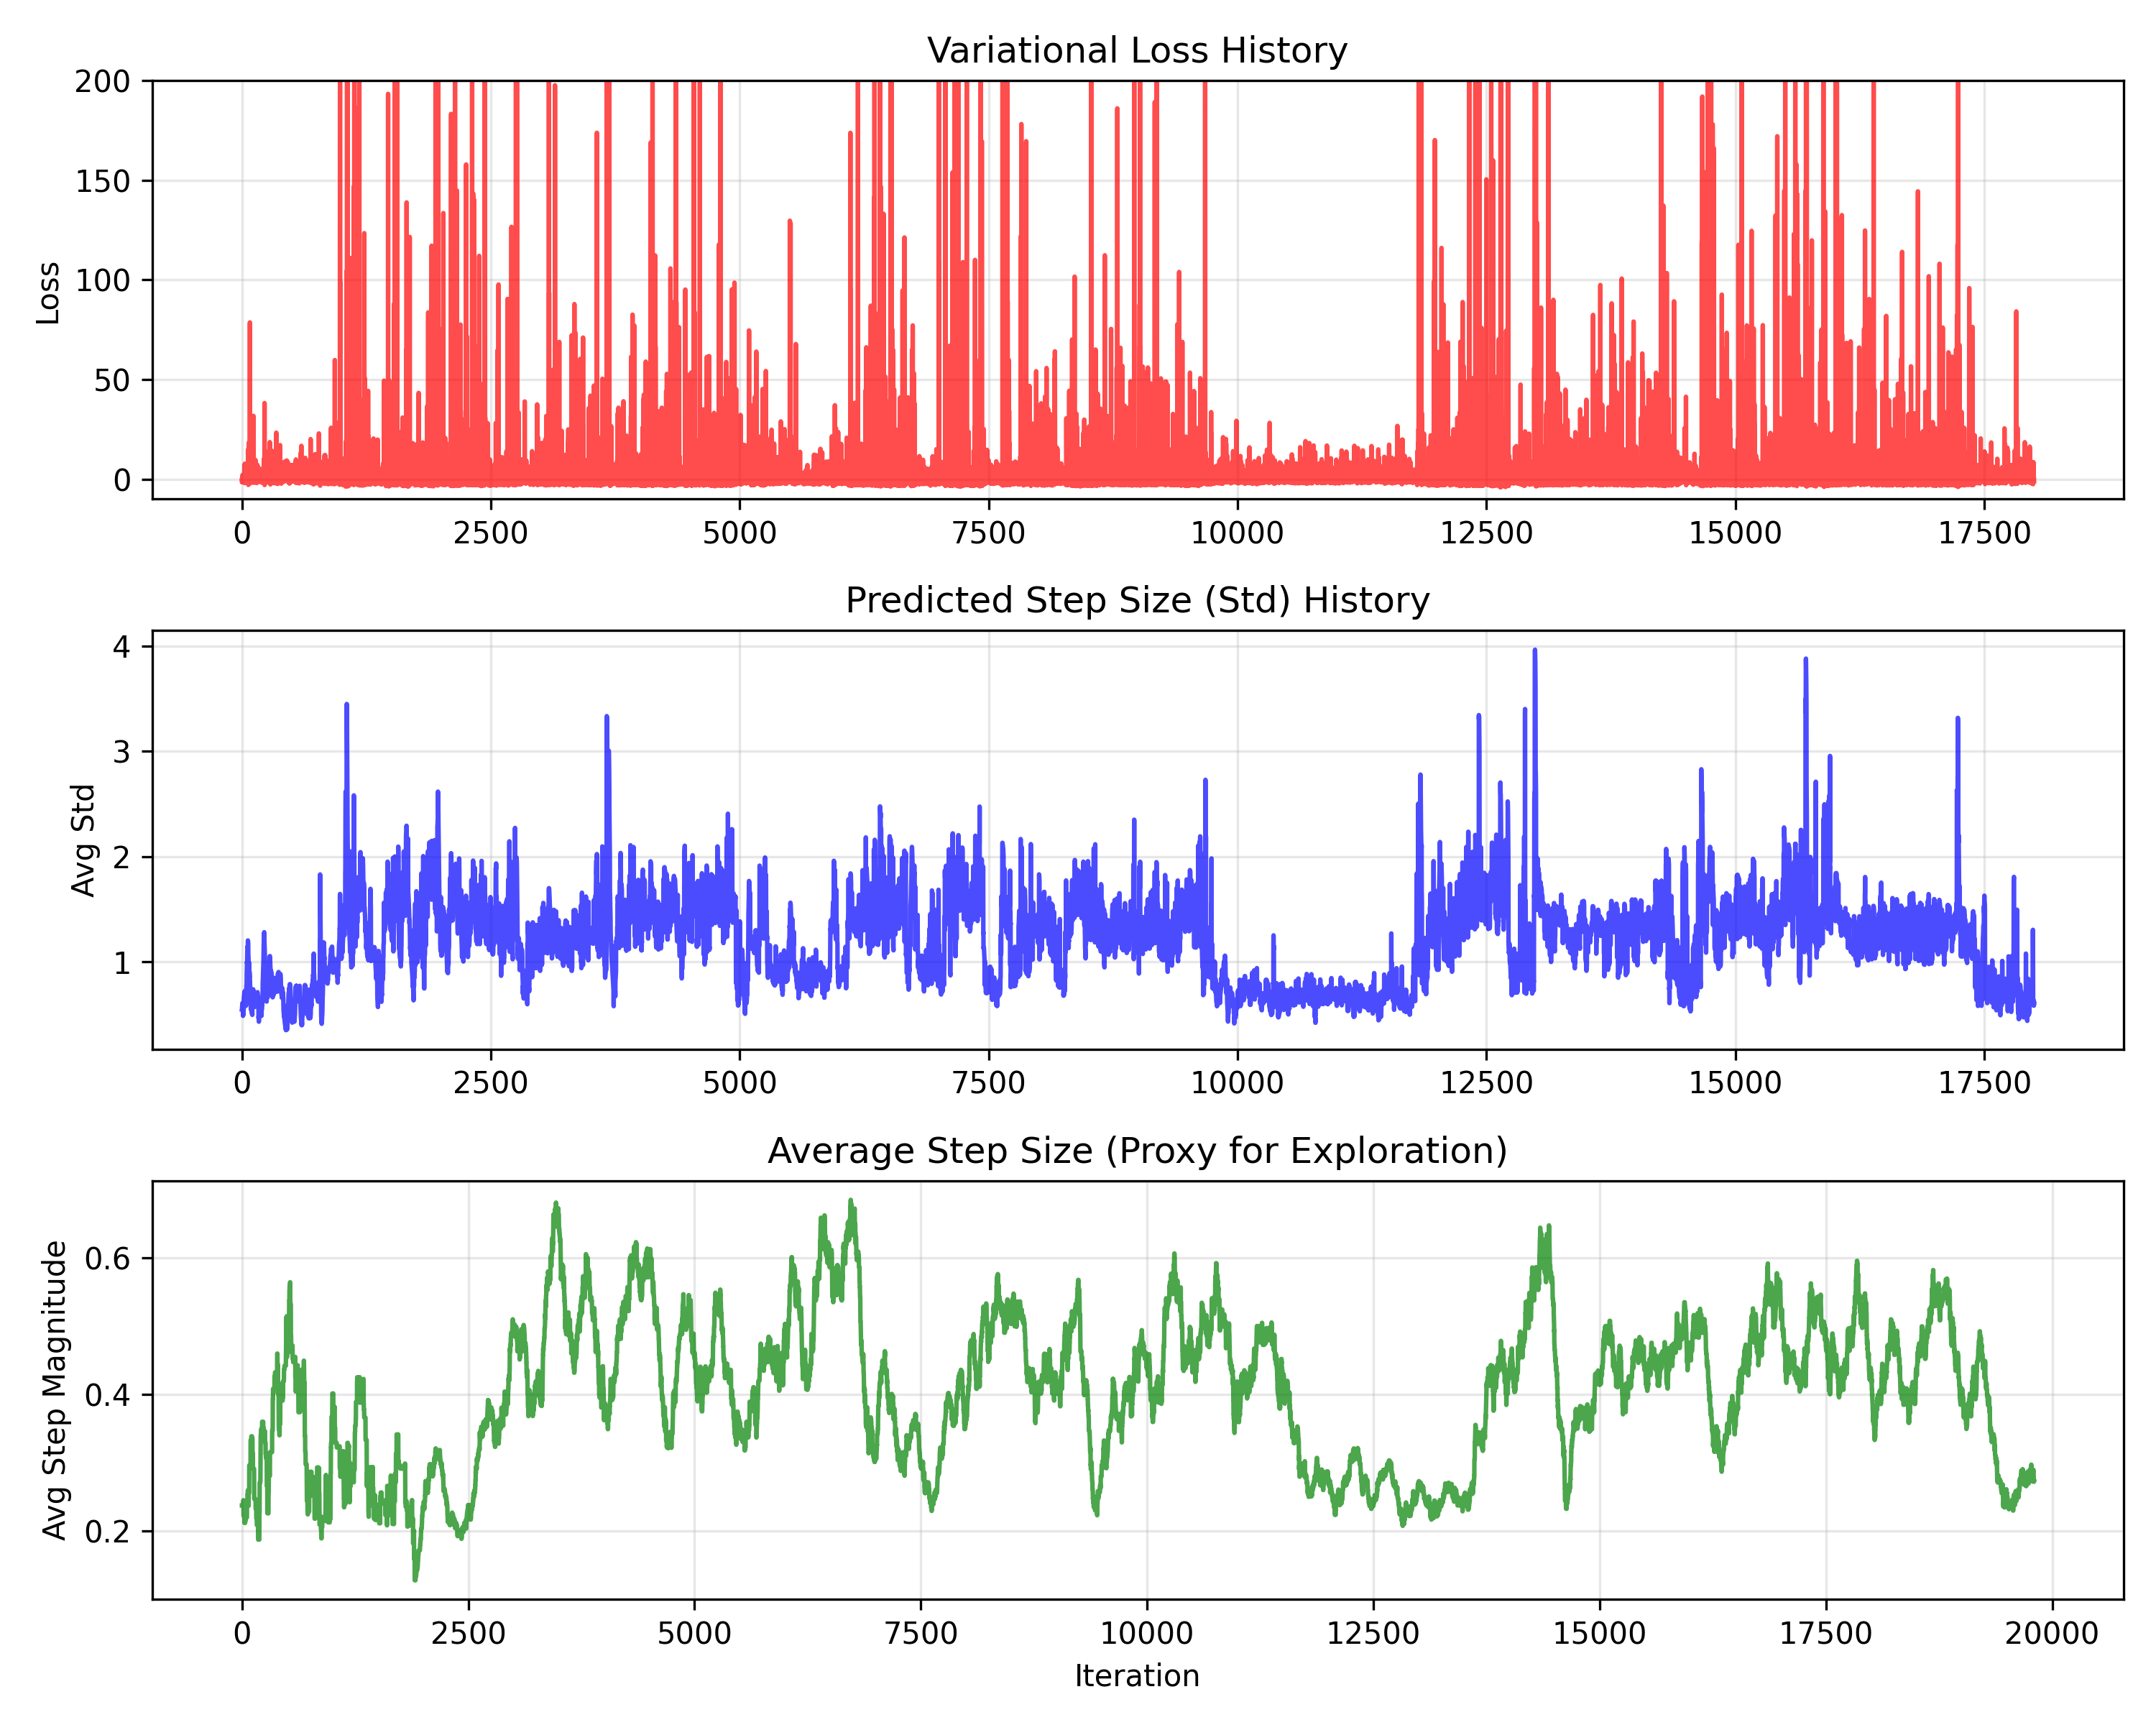
\includegraphics[width=0.5\textwidth]{../assets/variational_training_metrics.png}
        \caption{Loss History and Average Step Size}
    \end{figure}
    
    \begin{itemize}
        \item Loss is noisy due to online stochastic optimization.
        \item \textbf{Key Metric:} Predicted Step Size stabilizes.
        \item The network learns to adapt $\sigma$ based on location.
    \end{itemize}
\end{frame}

\begin{frame}{Interpreting the Learned Proposal}
    What did the network learn?
    
    \begin{columns}
        \column{0.5\textwidth}
        \begin{figure}
            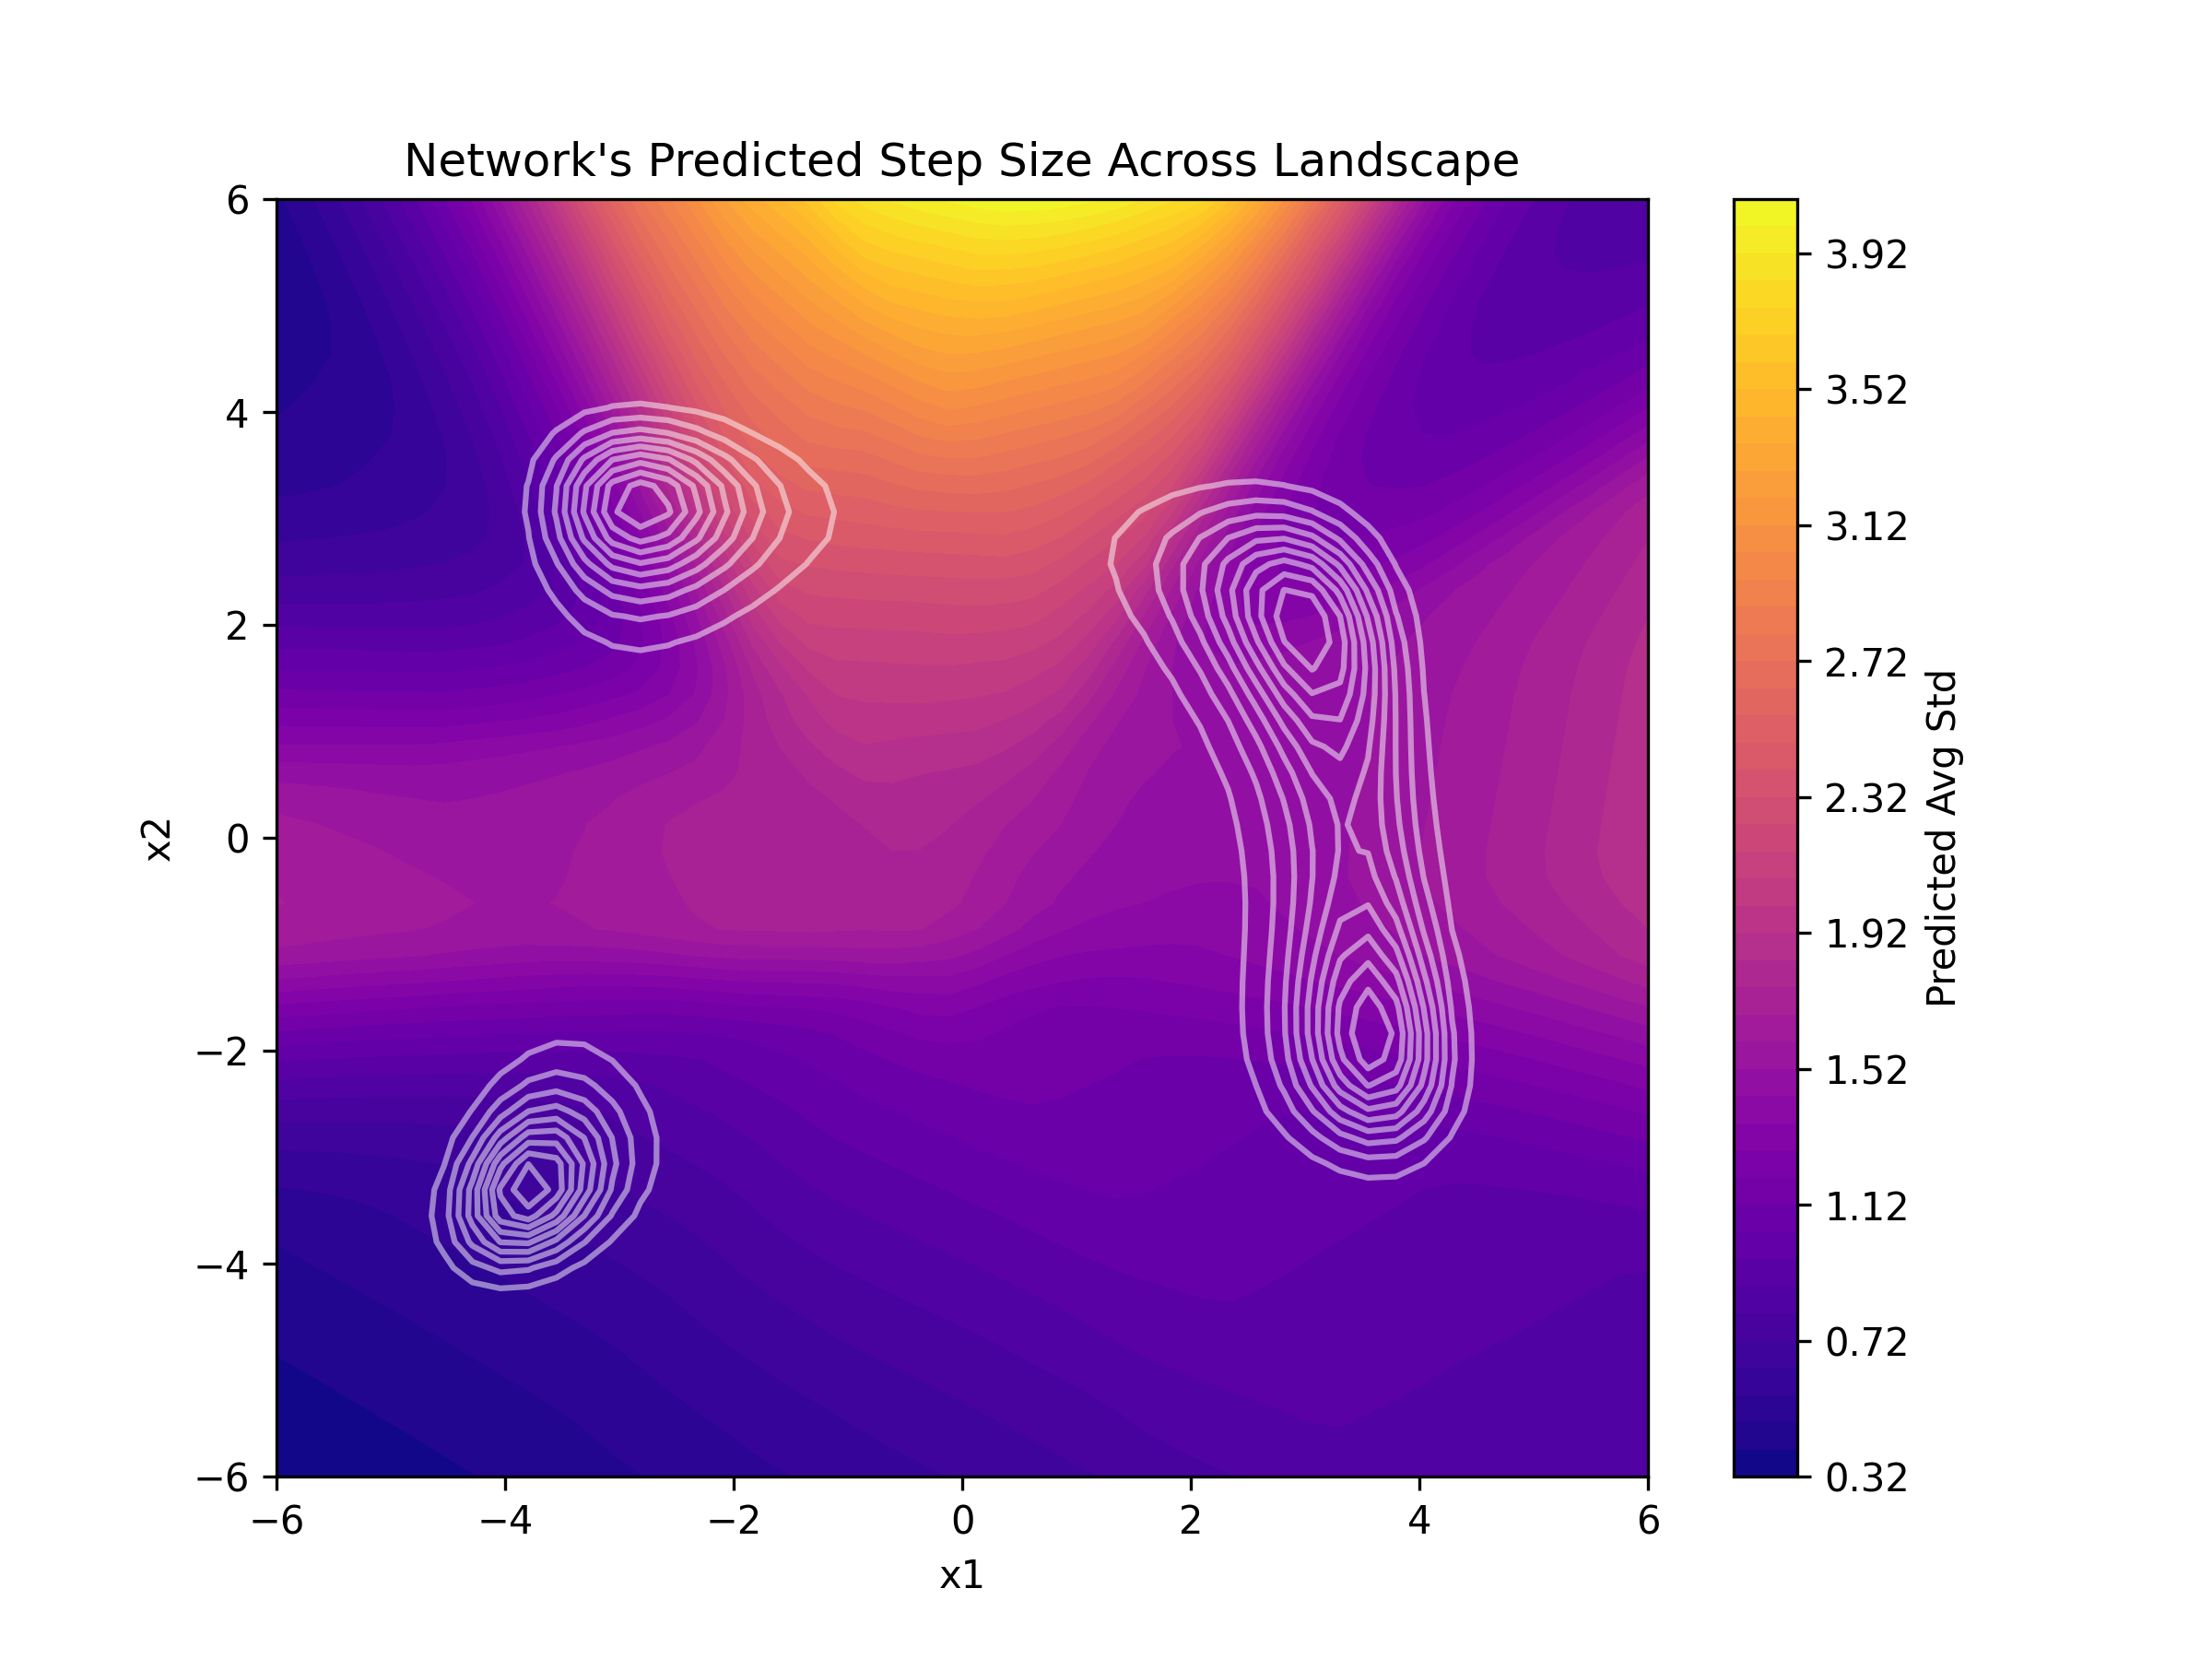
\includegraphics[width=\textwidth]{../assets/predicted_std_map.png}
            \caption{Predicted Step Size (Std)}
        \end{figure}
        
        \column{0.5\textwidth}
        \begin{figure}
            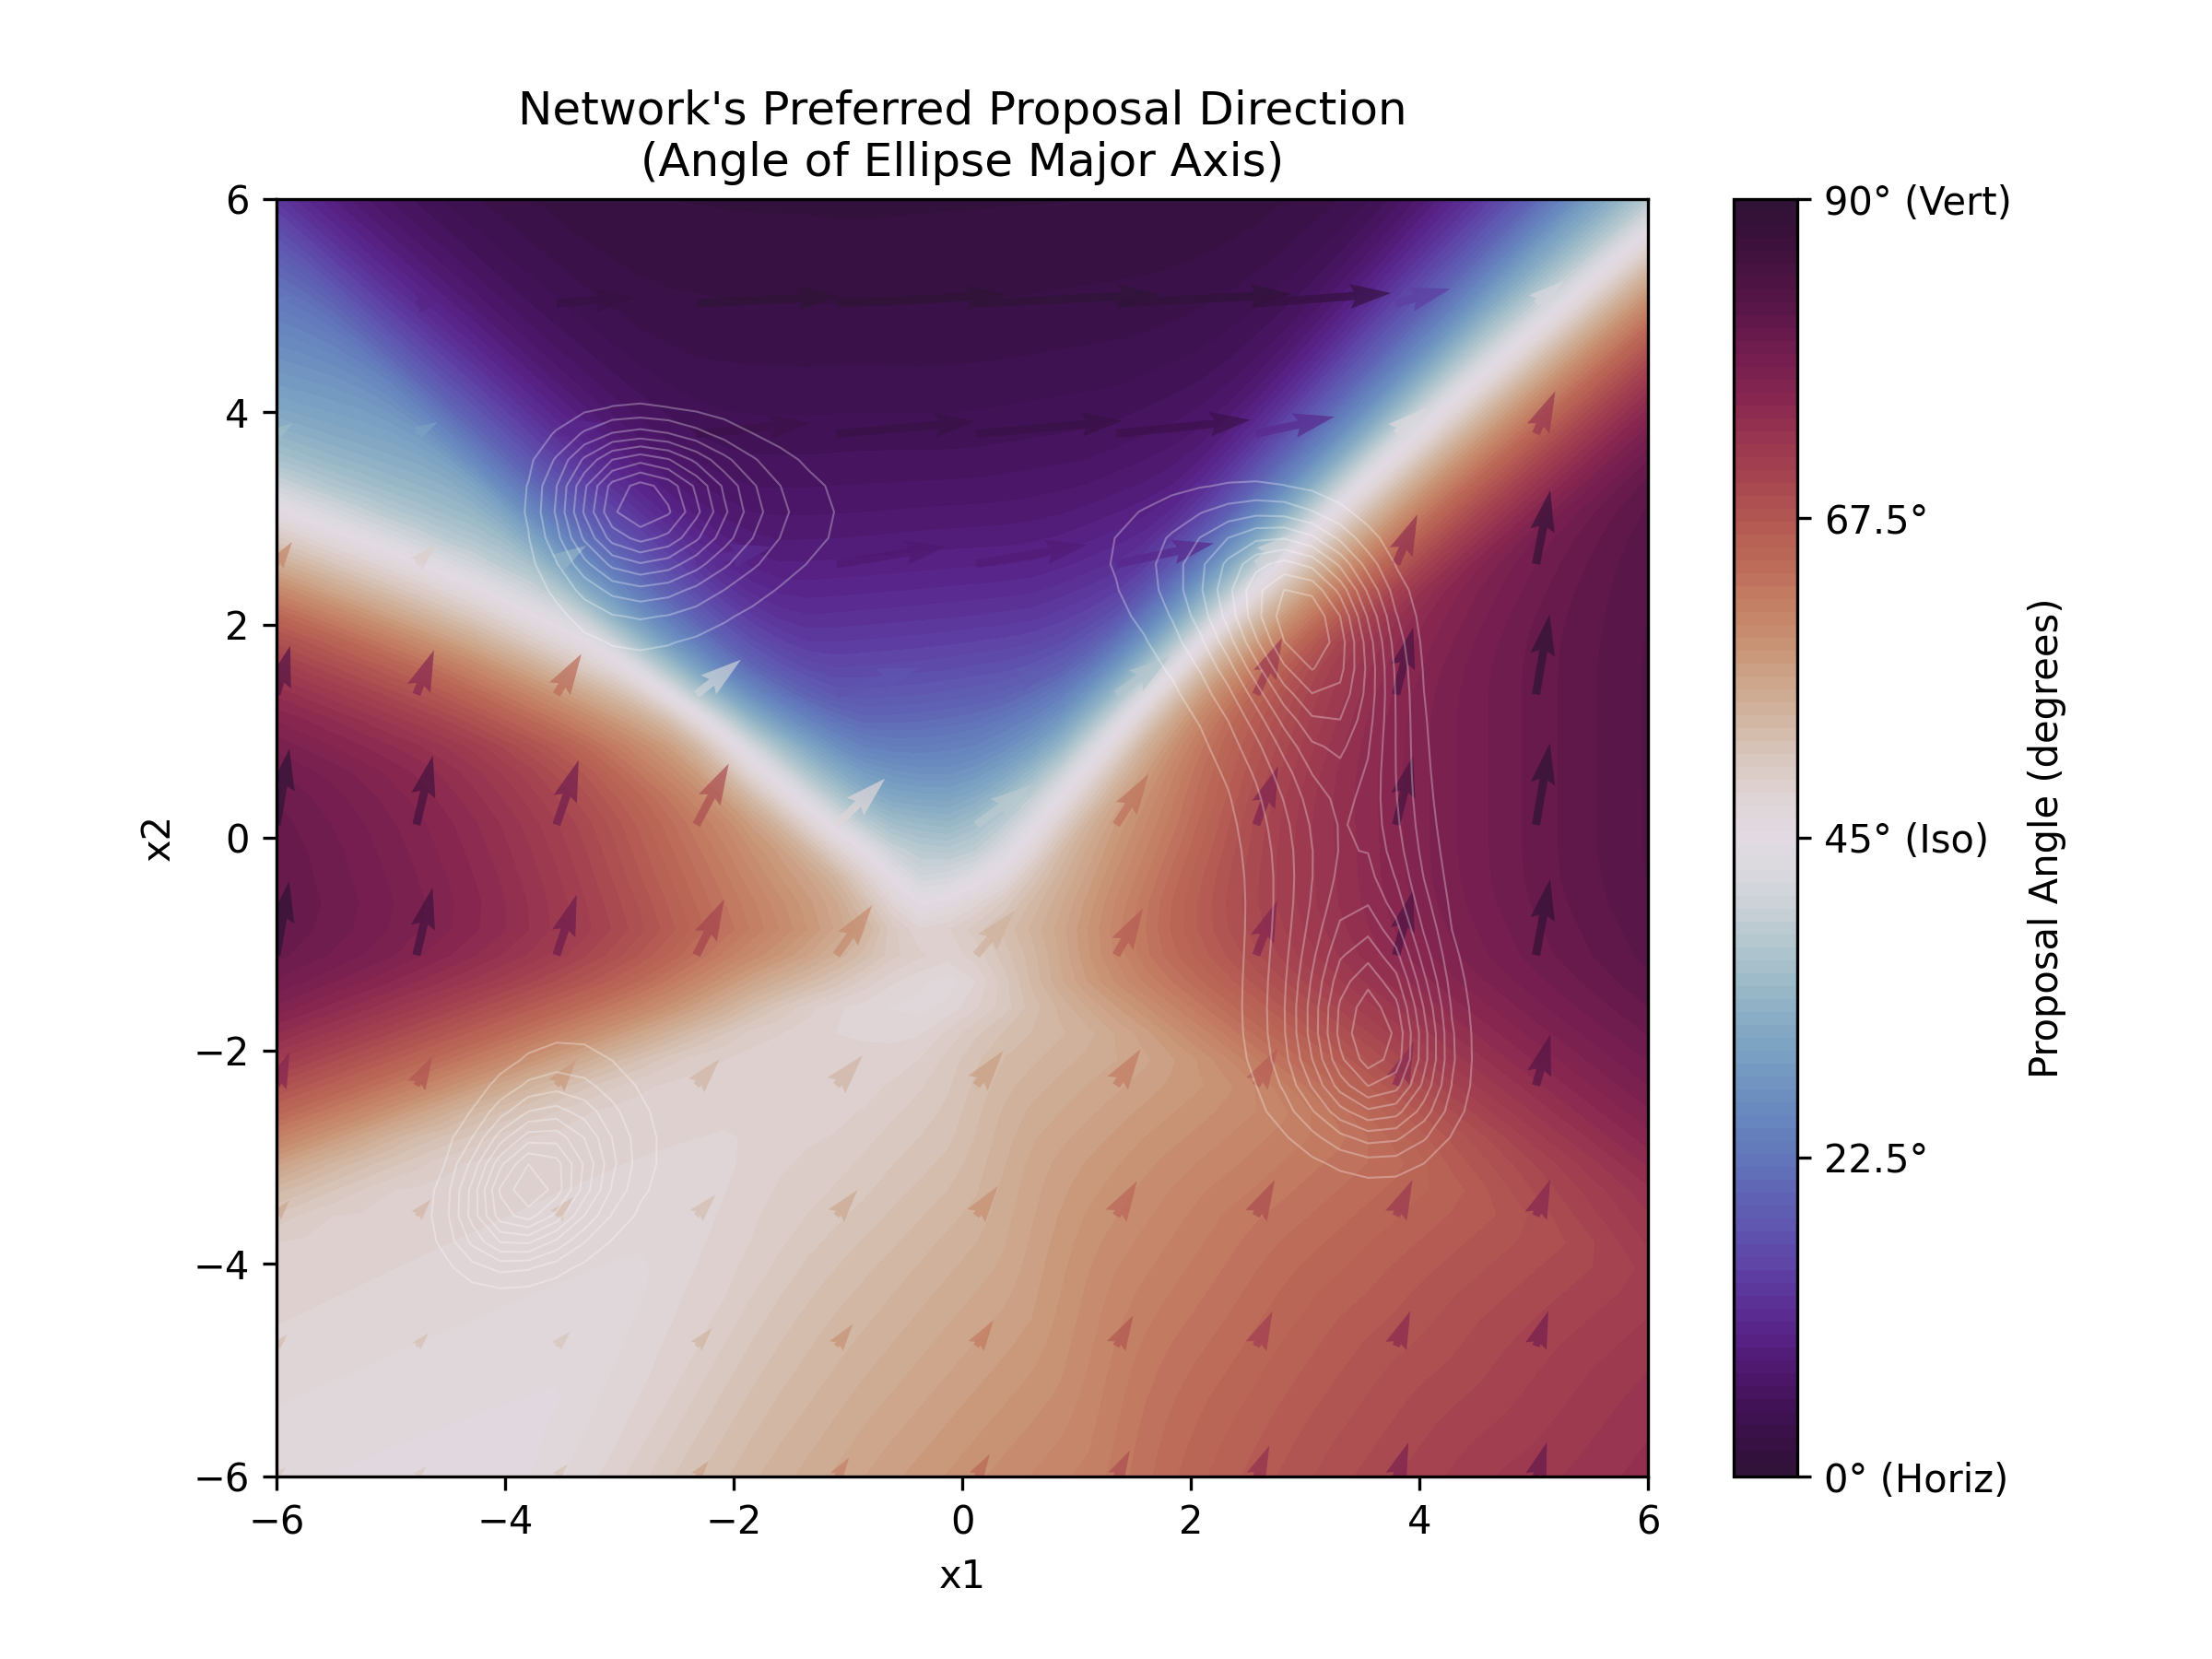
\includegraphics[width=\textwidth]{../assets/proposal_direction_map.png}
            \caption{Proposal Direction (Angle)}
        \end{figure}
    \end{columns}
    
    \begin{itemize}
        \item \textbf{Large Steps} in low-density valleys (fast traversal).
        \item \textbf{Small Steps} near high-density peaks (precise sampling).
        \item Directionality aligns with the geometry of the valleys.
    \end{itemize}
\end{frame}

\begin{frame}{Performance Comparison: Histograms}
    \textbf{Inference Run:} 6,000 iterations, Fixed Trained Model.
    
    \begin{figure}
        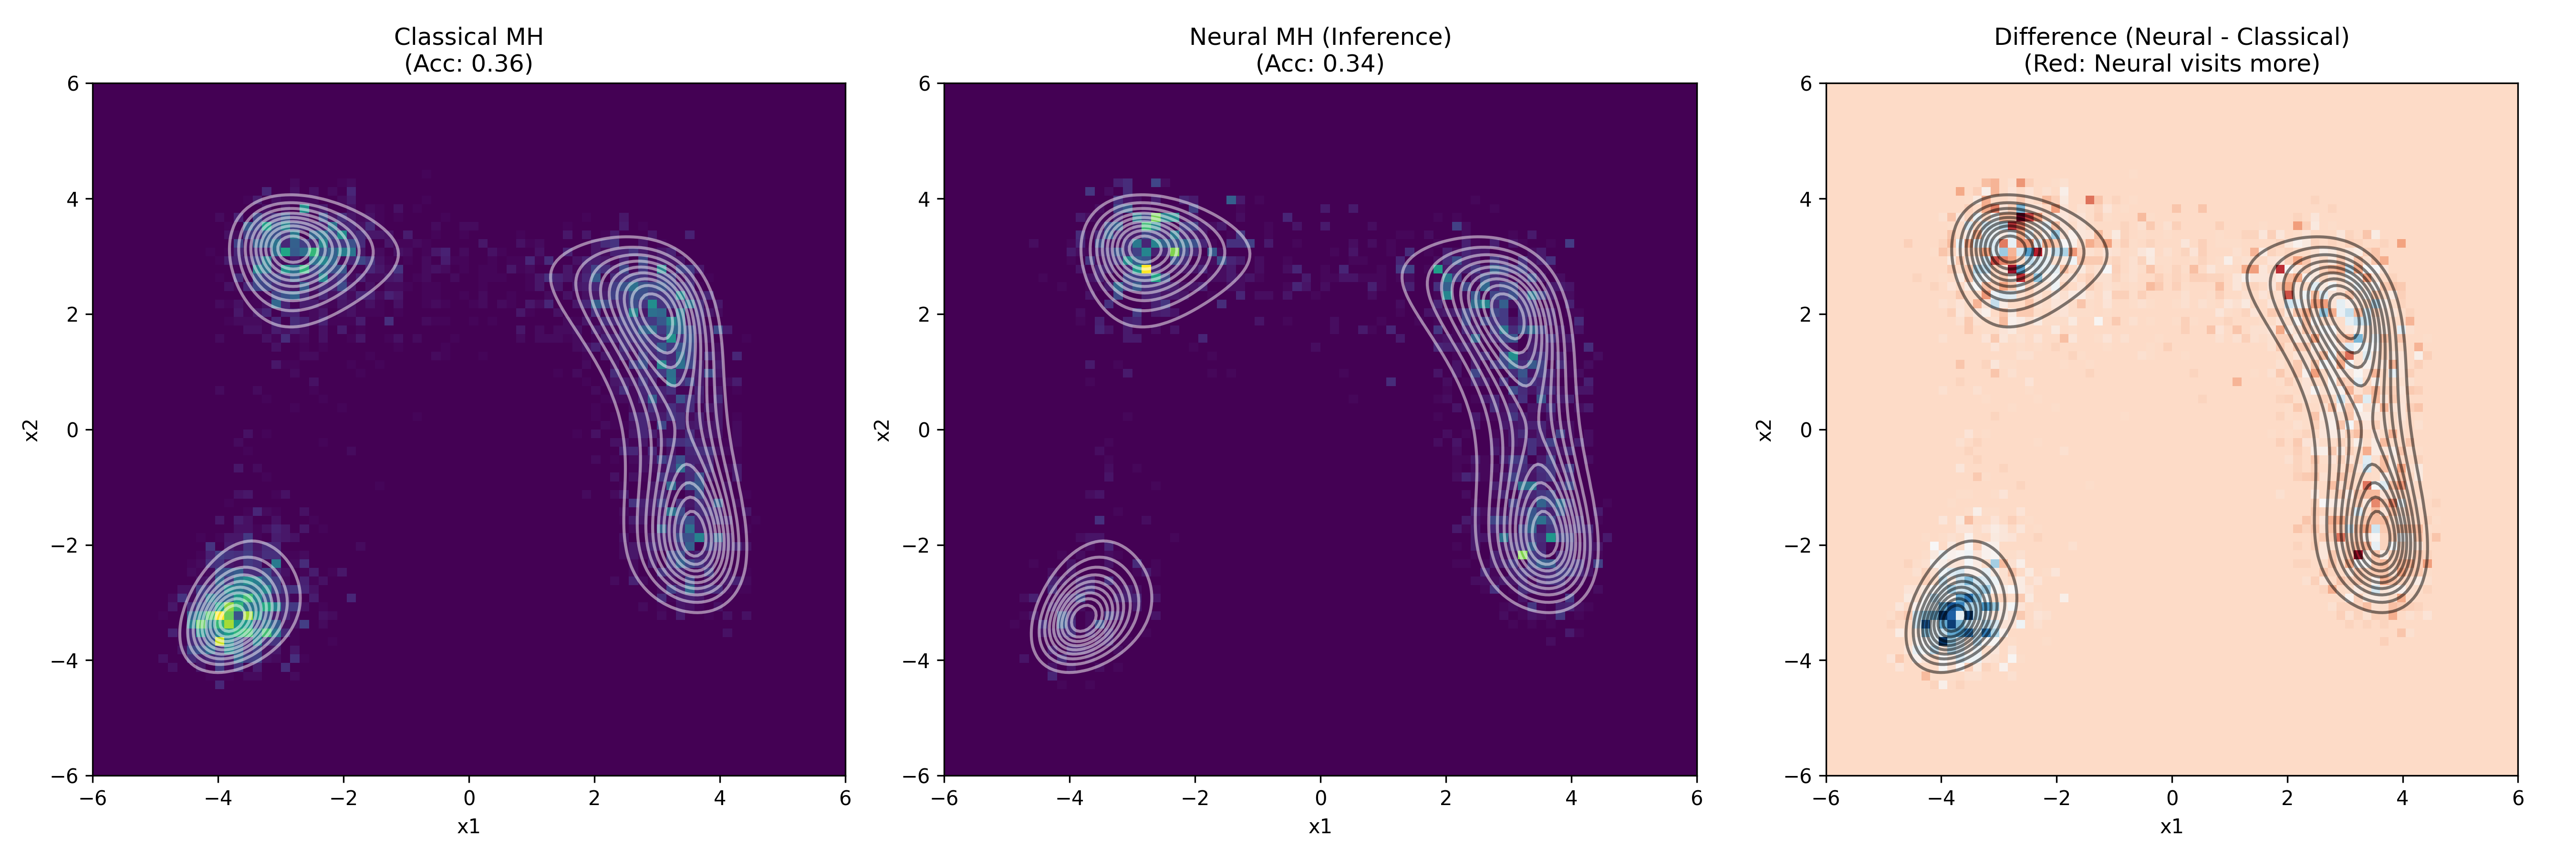
\includegraphics[width=0.9\textwidth]{../assets/histogram_comparison.png}
        \caption{Classical (Left) vs. Neural (Right) Sampling Distribution}
    \end{figure}
    
    \begin{itemize}
        \item Classical: Biased towards initial mode.
        \item Neural: Explores all 4 modes more uniformly.
    \end{itemize}
\end{frame}

\begin{frame}{Performance Comparison: Mode Occupancy}
    \textbf{Visualizing Mixing Behavior}
    
    \begin{figure}
        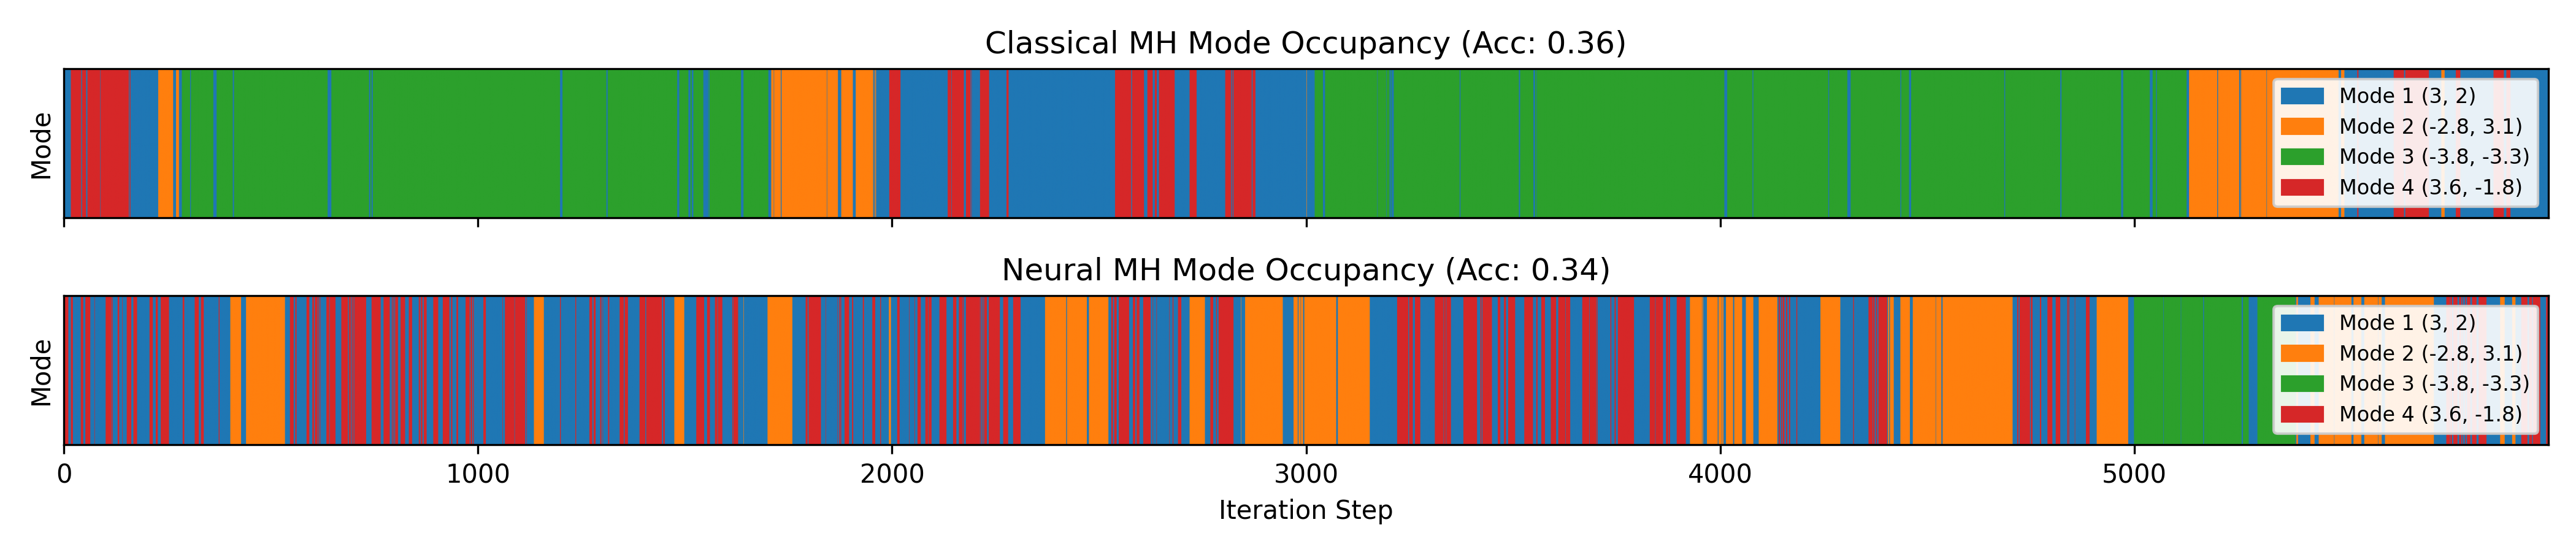
\includegraphics[width=\textwidth]{../assets/mode_occupancy_comparison.png}
        \caption{Mode Occupancy Plot (Color = Mode ID)}
    \end{figure}
    
    \begin{itemize}
        \item \textbf{Top (Classical):} Long solid blocks $\rightarrow$ Stuck in local modes.
        \item \textbf{Bottom (Neural):} Frequent color changes $\rightarrow$ Rapid mixing.
        \item Neural MH overcomes energy barriers effectively.
    \end{itemize}
\end{frame}

% ---------------------------------------------------------
% SECTION 4: Conclusion
% ---------------------------------------------------------
\section{Conclusion}

\begin{frame}{Conclusion and Future Work}
    \begin{itemize}
        \item \textbf{Summary:} We proposed a Neural MH algorithm that learns adaptive proposal variances.
        \item \textbf{Benefit:} Automates tuning and accelerates convergence in multi-modal landscapes.
        
        \vspace{0.3cm}
        
        \item \textbf{Limitations \& Future Work:}
        \begin{enumerate}
            \item \textbf{Training Stability:} Noisy loss requires careful hyperparameter tuning.
            \item \textbf{Covariance Structure:} Currently diagonal; future work could learn full correlations.
            \item \textbf{Dimensionality:} Tested on 2D; expected to scale well to higher dimensions where random walks fail.
            \item \textbf{Cost:} Higher cost per step (NN forward pass) but lower cost per effective sample.
        \end{enumerate}
    \end{itemize}
\end{frame}

\begin{frame}[allowframebreaks]{References}
    \begin{thebibliography}{99}

        \bibitem{mackay2003information}
        David J.C. MacKay (2003). 
        \newblock Information Theory, Inference, and Learning Algorithms.

        \bibitem{Hastings1970MonteCS}
        W. K. Hastings (1970).
        \newblock Monte Carlo Sampling Methods Using Markov Chains and Their Applications.
        \newblock \emph{Biometrika}, 57, 97--109.

        \bibitem{HuntSmith2023AcceleratingMC}
        N. T. Hunt-Smith, Wally Melnitchouk, F. Ringer, N. Sato, A. W. Thomas, M. J. White (2023).
        \newblock Accelerating Markov Chain Monte Carlo sampling with diffusion models.
        \newblock \emph{Comput. Phys. Commun.}, 296, 109059.

        \bibitem{Turner2018MetropolisHastingsGA}
        Ryan D. Turner, Jane Hung, Yunus Saatci, Jason Yosinski (2018).
        \newblock Metropolis-Hastings Generative Adversarial Networks.
        \newblock In \emph{International Conference on Machine Learning}.

    \end{thebibliography}
\end{frame}

\end{document}